% https://tex.stackexchange.com/a/762321

\documentclass[tikz,border=5pt]{standalone}
\usetikzlibrary{arrows.meta}

\makeatletter
\newcommand\dualharpoon{}
\newcommand\dualharpoon@aux{}
\newcommand\dualharpoon@noaux{}

\protected\def\dualharpoon{%
  \@ifnextchar[\dualharpoon@aux\dualharpoon@noaux
}

\protected\def\dualharpoon@noaux{%
  \dualharpoon@aux[]%
}

\long\protected\def\dualharpoon@aux[#1]#2#3#4#5{%
  \path (#4.center);
  \pgfgetlastxy{\temp@ax}{\temp@ay}
  \path (#5.center);
  \pgfgetlastxy{\temp@bx}{\temp@by}
  \pgfmathsetmacro\temp@angle{atan2(\temp@by-\temp@ay,\temp@bx-\temp@ax)}

  \draw[-foo,mystyle]
    (#4.{\temp@angle - 10}) --
    node[
      midway,
      sloped,
      allow upside down,
      above=5pt,
      inner sep=0pt,
      #1
    ] {#2}
    (#5.{190+\temp@angle});

  \draw[foo-,mystyle]
    (#4.{\temp@angle + 10}) --
    node[
      midway,
      sloped,
      allow upside down,
      below=5pt,
      inner sep=0pt,
      #1
    ] {#3}
    (#5.{170+\temp@angle});
}
\makeatother

\begin{document}

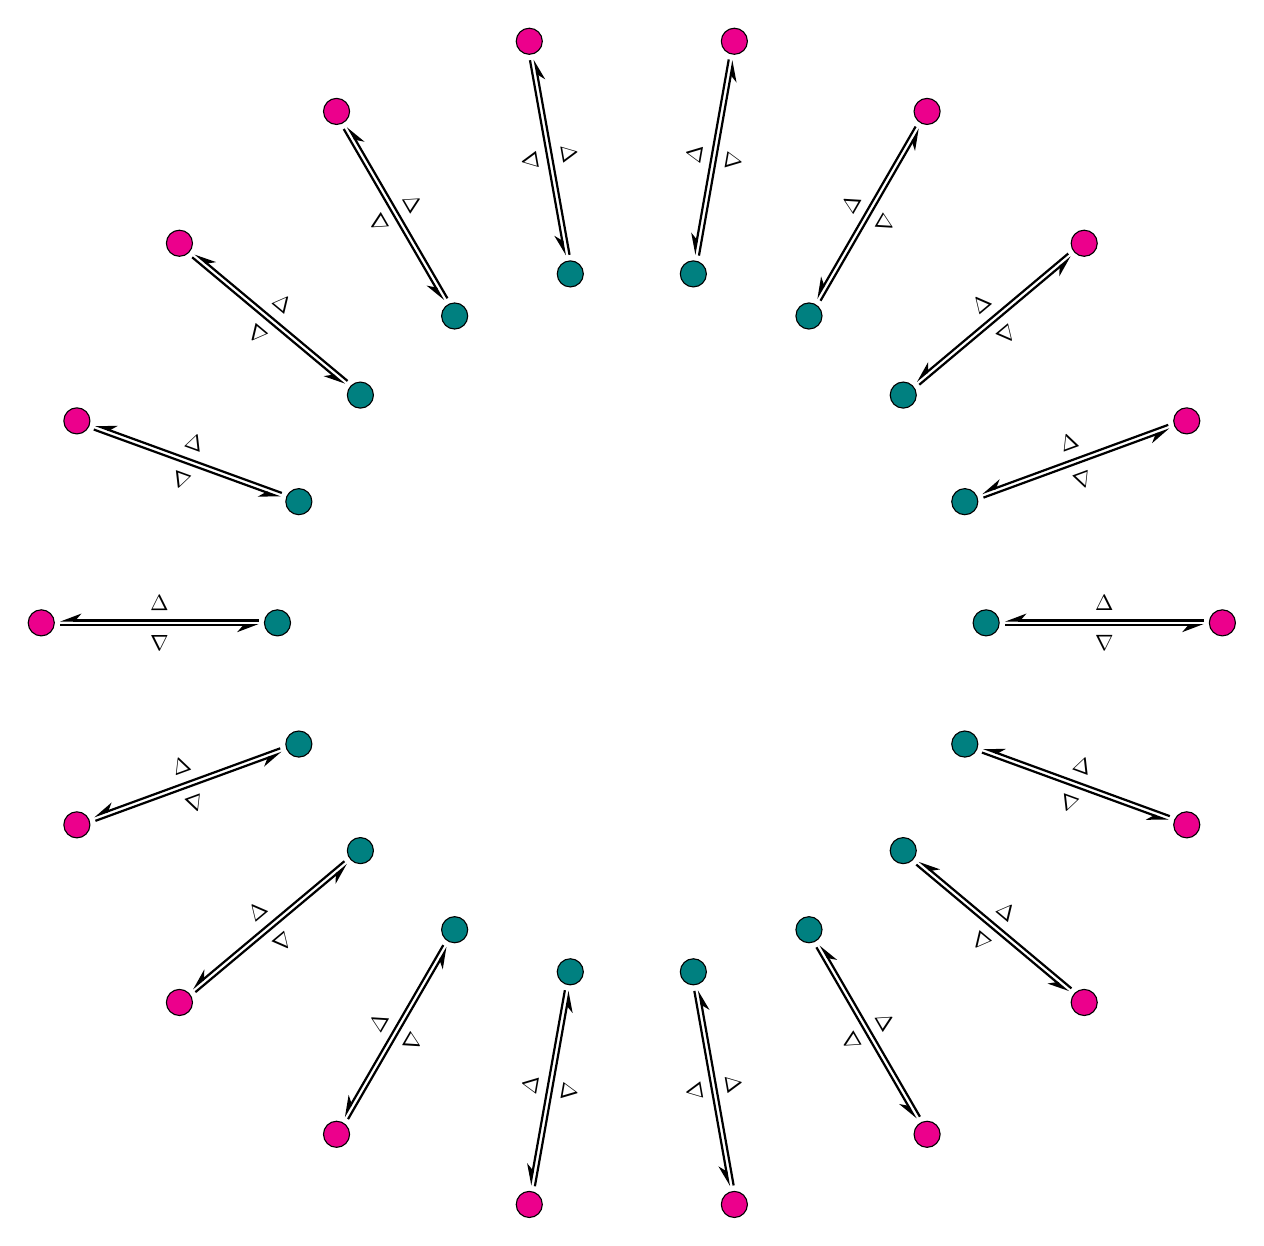
\begin{tikzpicture}[
  foo/.tip={Stealth[harpoon,swap]},
  scale=1.5,
  mystyle/.style={
    thick,
    shorten >=2pt,
    shorten <=2pt
  }
]
  \foreach \i in {0,20,...,340}{
    \node[draw,circle,fill=teal] (In-\i) at (\i:3) {};
    \node[draw,circle,fill=magenta] (Out-\i) at (\i:5) {};
    \dualharpoon[scale=.8]{$\Delta$}{$\nabla$}{In-\i}{Out-\i}
  }
\end{tikzpicture}

\end{document}
